\subsubsection{Umgang mit gebrochenen Funktionen}

\begin{figure}[H]
	\centering
	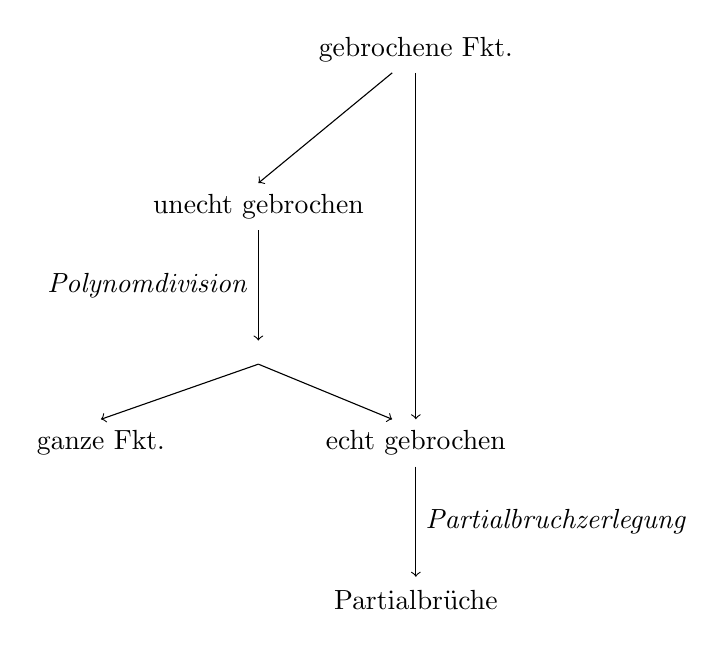
\begin{tikzpicture}
		\node[] at (0, 1) {gebrochene Fkt.};
		\node[] at (-2,-1) {unecht gebrochen};
		\node[left] at (-2, -2) {\textit{Polynomdivision}};
		\node[] at (-4, -4) {ganze Fkt.};
		\node[] at (0, -4) {echt gebrochen};
		\node[right] at (0, -5) {\textit{Partialbruchzerlegung}};
		\node[] at (0, -6) {Partialbrüche};

		\draw[->] ( -0.3, 0.7) -- (-2,-0.7);
		\draw[->] ( 0, 0.7) -- ( 0,-3.7);
		\draw[->] ( 0, -4.3) -- ( 0,-5.7);
		\draw[->] (-2, -1.3) -- (-2,-2.7);
		\draw[->] (-2, -3)   -- (-4,-3.7);
		\draw[->] (-2, -3)   -- (-0.3,-3.7);
	\end{tikzpicture}
	\caption{Umgang mit gebrochenen Funktionen}\label{fig:gebrochene_funktionen_graph}
\end{figure}
